% ============================================
% §5 Methodology
% ============================================
\section{Experimental Methodology}
\label{sec:methodology}

The evaluation is organized around three empirical questions. At a
single difficulty, which prompt and memory layers matter? If a frozen
$L_4{+}L_5$ stack is moved to another backbone, does it still help?
When postrun writing is allowed, how far does the agent climb on the
Ascension ladder?

\subsection{\texorpdfstring{The 5-condition decomposition at fixed $A_0$}{The 5-condition decomposition at fixed A0}}
\label{sec:methodology:fivecond}

\begin{figure*}[t]
  \centering
  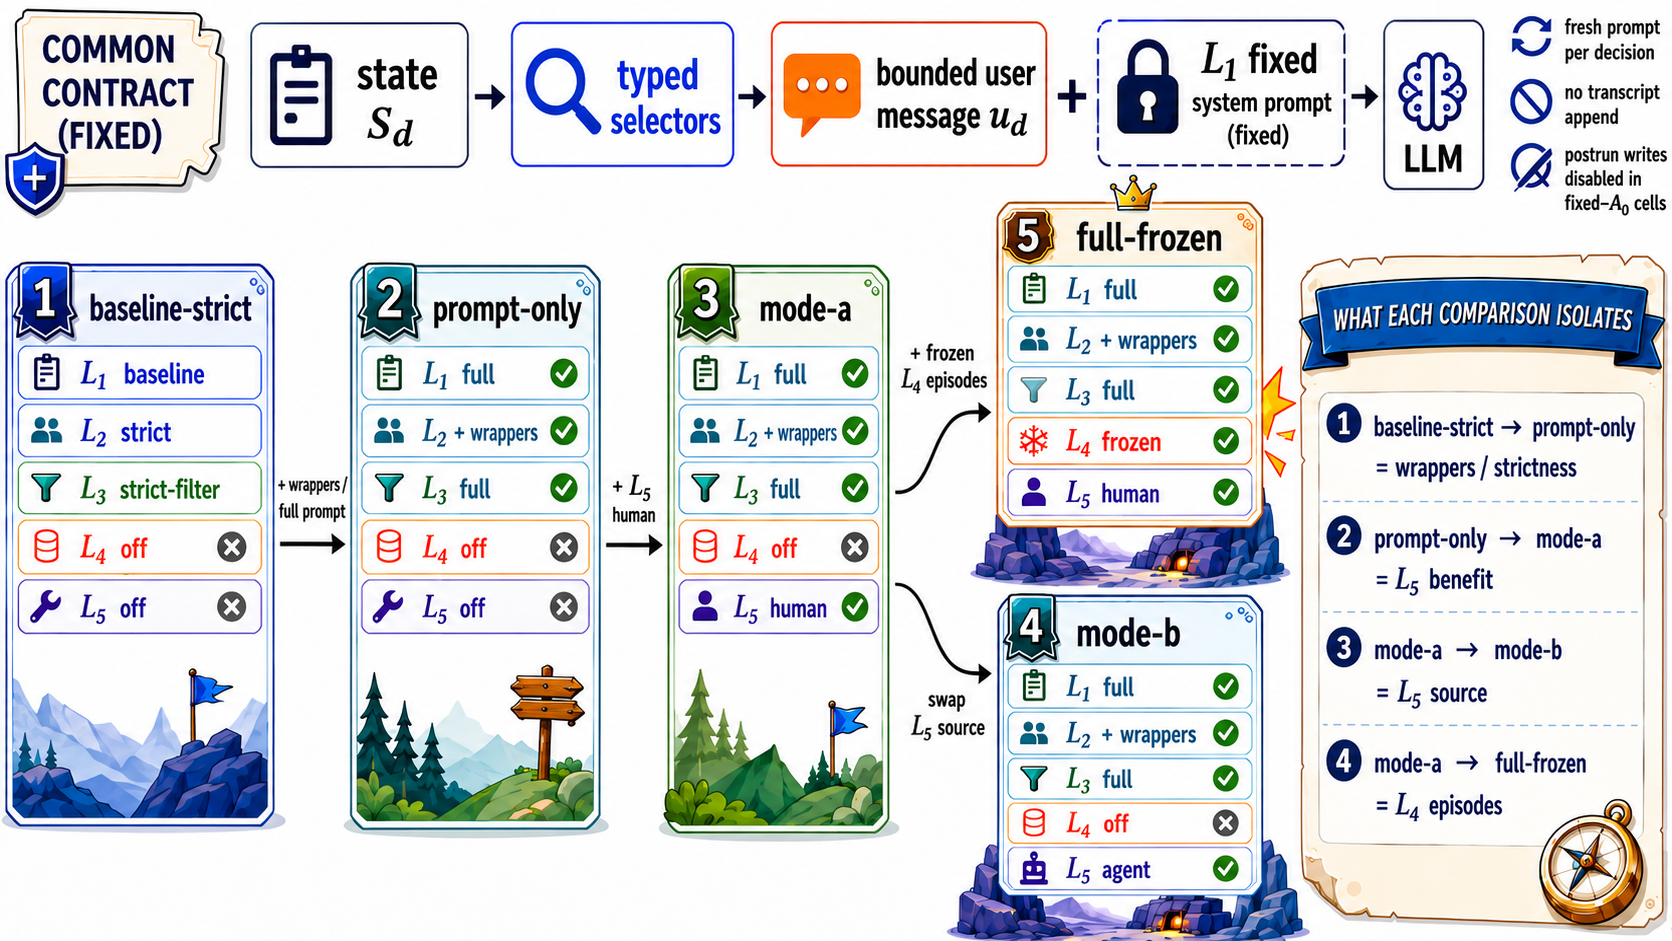
\includegraphics[width=\linewidth]{figures/v2/pro_fig3.png}
  \caption{Fixed-$A_0$ ablation surface under the bounded-memory
  contract: five cells share a common contract and adjacent bars are
  organized by a named ablation axis. Not every neighboring pair is a
  single-mechanism isolation---e.g.\ baseline-strict to prompt-only
  changes the prompt-package/strictness group rather than one isolated
  mechanism. Frozen stores at SHA \texttt{1888a62}.}
  \label{fig:fivecond-surface}
\end{figure*}

The fixed-$A_0$ study is a five-cell decomposition, not a full
factorial grid (Figure~\ref{fig:fivecond-surface}).
\texttt{baseline-strict} uses the baseline prompt with no memory,
no skills, no strategic thread, and no combat-conversation wrapper;
it also applies the strict knowledge/hint filter. \texttt{prompt-only}
keeps the full prompt and conversation helpers but disables $L_4$ and
$L_5$. \texttt{mode-a} adds human-authored $L_5$ seed bodies.
\texttt{mode-b-frozen} replaces those bodies with stub-template-filled
$L_5$ bodies. \texttt{full-frozen} adds the frozen $L_4$ episodic
store to Mode~A. In all five cells, postrun and evolution writes are
disabled, anchoring the active stores at SHA \texttt{1888a62}.

\subsection{Cross-backbone probe and auto-mode ladder}
\label{sec:methodology:crossmodel}

The frozen $L_4{+}L_5$ stack was derived from Gemini~3.1~Pro
trajectories. To test how backbone-specific that stack is, we run
\texttt{baseline-strict} and \texttt{full-frozen} at $A_0$ on three
backbones: Qwen~3.6~27B, DeepSeek~V4~Pro, and Gemini~3.1~Pro. The
Qwen and DeepSeek probe adds $N{=}5$ completed games per
backbone-cell; the Gemini rows reuse the corresponding fixed-$A_0$
cells as anchors. We report this probe separately from the headline
ablation; Appendix~\ref{app:configs} lists the denominator rules.

The auto-mode ladder uses a different protocol. After a victory at
$A_n$, the next run attempts $A_{n+1}$; after a defeat, it retries
$A_n$. This stream measures the observed climb endpoint, whereas the
fixed-$A_0$ matrix measures reliability at one difficulty.

\subsection{Statistical protocol}
\label{sec:methodology:stats}

Cell-level win rates use Wilson 95\% confidence intervals
\citep{wilson1927}. Continuous scores (Eq.~\ref{eq:score}) use
5{,}000-bootstrap 95\% intervals \citep{efron1979}. The descriptive pooled scaffolded row uses an exact
Clopper--Pearson interval and is labeled as such. For the headline
fixed-$A_0$ table, we take the first ten completed games per
condition by start time, giving a balanced 50-game comparison. For
context, recent LLM-agent game evaluations typically report
3--25 episodes per condition---e.g., $3$ trials per cell in Voyager
\citep{voyager2023} and 10--25 seeds per task in BALROG
\citep{balrog2024}---so the present balanced $5\!\times\!10$ subset
sits at or above the comparable range while keeping completed-run
denominators interpretable. Completed games are the denominator
throughout. Additional completed games in the archive remain in
their diagnostic streams and are not pooled into the fixed-$A_0$
estimate. Score-based qualitative comparisons were also checked
after perturbing the $52/3$ coefficient by $\pm 10\%$; win-rate
intervals are unaffected.

\subsection{Reproducibility and release contents}
\label{sec:methodology:repro}

The public release includes the completed-run archive, condition
tags, analysis scripts, frozen memory/skill snapshots, and
representative prompt records needed to recompute the reported win
rates \citep{deal-checklist-2025,liu-versioning-2025}. The same
archive defines the natural next matched experiment: an
accumulating-context condition implemented in the same codebase with
the same run protocol and scoring scripts. Scope limits that affect
interpretation are noted where they arise and collected in the
Limitations section.
